%%%%%%%%%%%%%%%%%%%%%%%%%%%%%%%%%%%%%%%%%%%%%%%%%%%%%%%%%%%%%%%%
%                                                              %
%                                                              %
% Macallyster S. Edmondson                                     %
%                                                              %
% ECE351-53                                                    %
%                                                              %
% Lab #11                                                      %
%                                                              %
% 04/12/2022                                                   %
%                                                              %
% Straightforward layout, broken into sections, uses many      %
% common libraries. Note, Hyperlinks are not highlighted.      %
%                                                              %
%%%%%%%%%%%%%%%%%%%%%%%%%%%%%%%%%%%%%%%%%%%%%%%%%%%%%%%%%%%%%%%%

%%%%%%%%%%%%%%%%%%%%%%%%%%%%%%%%%%%%%%%%%%%
%%% DOCUMENT PREAMBLE %%%
\documentclass[12pt]{report}
\usepackage[english]{babel}
%\usepackage{natbib}
\usepackage{url}
\usepackage[utf8x]{inputenc}
\usepackage{amsmath}
\usepackage{graphicx}
\graphicspath{{./images/}}
\usepackage{parskip}
\usepackage{fancyhdr}
\usepackage{vmargin}
\usepackage{listings}
\usepackage[hidelinks]{hyperref}
\usepackage{xcolor}
\usepackage[nodayofweek]{datetime}
\usepackage[section]{placeins}
\usepackage{pdfpages}
\usepackage{float}
\definecolor{codegreen}{rgb}{0,0.6,0}
\definecolor{codegray}{rgb}{0.5,0.5,0.5}
\definecolor{codeblue}{rgb}{0,0,0.95}
\definecolor{backcolour}{rgb}{0.95,0.95,0.92}
\lstdefinestyle{mystyle}{
backgroundcolor=\color{backcolour},
commentstyle=\color{codegreen},
keywordstyle=\color{codeblue},
numberstyle=\tiny\color{codegray},
stringstyle=\color{codegreen},
basicstyle=\ttfamily\footnotesize,
breakatwhitespace=false,
breaklines=true,
captionpos=b,
keepspaces=true,
numbers=left,
numbersep=5pt,
showspaces=false,
showstringspaces=false,
showtabs=false,
tabsize=2
}
\lstset{style=mystyle}
\setmarginsrb{3 cm}{2.5 cm}{3 cm}{2.5 cm}{1 cm}{1 cm}{1 cm}{1.5 cm}
\title{Lab \#12 Report}
% Title
\author{Macallyster S. Edmondson}
% Author
\newdate{date}{26}{04}{2022}
\date{\longdate\displaydate{date}}
% Date
\makeatletter
\let\thetitle\@title
\let\theauthor\@author
\let\thedate\@date
\makeatother
\pagestyle{fancy}
\fancyhf{}
\rhead{\theauthor}
\lhead{\thetitle}
\lfoot{Page: \thepage}
\rfoot{\thedate}
\fancypagestyle{customplain}{ %Used for default pages with plain style to keep overall document consistency
  \fancyhf{}
  \renewcommand{\headrulewidth}{0pt} %Remove bar from top of page
  \lfoot{Page: \thepage}
}
\fancypagestyle{titlepage}{ %Used for default pages with plain style to keep overall document consistency
  \fancyhf{}
  \renewcommand{\headrulewidth}{0pt} %Remove bar from top of page
  \cfoot{\thedate}
}
\fancypagestyle{customblank}{ %Used for default pages with plain style to keep overall document consistency
  \fancyhf{}
  \renewcommand{\headrulewidth}{0pt} %Remove bar from top of page
}
%%%%%%%%%%%%%%%%%%%%%%%%%%%%%%%%%%%%%%%%%%%%
\begin{document}
%%%%%%%%%%%%%%%%%%%%%%%%%%%%%%%%%%%%%%%%%%%%%%%%%%%%%%%%%%%%%%%%%%%%%%%%%%
%%%%%%%%%%%%%%%
\begin{titlepage}\thispagestyle{titlepage}
\centering
%\vspace*{0.5 cm}

\includegraphics[scale = 0.12]{univ-logo.png}\\[1.0 cm]
%University of Idaho
\begin{center}    \textsc{\Large   ECE 351 - Section \#53 }\\[2.0 cm]
\end{center}% University Name

%Lab Report
\rule{\linewidth}{0.2 mm} \\[0.4 cm]
{ \huge \bfseries \thetitle}\\
\rule{\linewidth}{0.2 mm} \\[0.5 cm]
\textsc{\Large Filter Design }\\[1.5 cm] % Course 
\begin{minipage}{0.4\textwidth}
\begin{flushleft} \large
\emph{Submitted To:}\\
Kate Antonov\\ \small
University of Idaho\\
kantonov@uidaho.edu\\
\hfill
\end{flushleft}
\end{minipage}~
\begin{minipage}{0.4\textwidth}
\begin{flushright} \large
\emph{Submitted By :} \\
\theauthor \\ \small
University of Idaho\\
edmo7033@vandals.uidaho.edu\\
\href{http://github.com/mac-edmondson}{github.com/mac-edmondson}\\
\end{flushright}
\end{minipage}\\[2 cm]
\vfill
\end{titlepage}
%%%%%%%%%%%%%%%%%%%%%%%%%%%%%%%%%%%%%%%%%%%%%%%%%%%%%%%%%%%%%%%%%%%%%%%%%%
%%%%%%%%%%%%%%%
\tableofcontents\thispagestyle{customplain}
\pagebreak
%%%%%%%%%%%%%%%%%%%%%%%%%%%%%%%%%%%%%%%%%%%%%%%%%%%%%%%%%%%%%%%%%%%%%%%%%%
%%%%%%%%%%%%%%%
\renewcommand{\thesection}{\arabic{section}}
\section{Introduction}
The goal of this lab was to take many of the concepts taught throughout this course and apply them to a practical
application. More specifically, we used concepts taught throughout this course to filter a positioning feedback
signal for an aircraft. The data on the signal is contained in the frequency range of $1.8\: kHz \leq f \leq 2.0\: kHz$.
Significant noise exists in the transmitted signal at higher frequencies due to a shared ground of the positioning
system and a switching amplifier. Low frequency vibrations also exist on the signal due to a building ventilation
system on the receiving end of the signal. A filter was designed to isolate the frequency range of the original signal.

This lab was completed using\textit{Python} through the \textit{Spyder-IDE}. The packages used in the completion 
of this lab were \texttt{numpy} for definitions of mathematical functions, \texttt{matplotlib.pyplot} to plot outputs 
of functions, \texttt{scipy.signal} \& \texttt{control} to compute the frequency response of a digital filter, 
\texttt{scipy.fftpack} to perform Fast Fourier Transform operations, and \texttt{pandas} to import signal data
from a CSV file.

All code for this lab, including this report, can be found on \href{http://github.com/mac-edmondson}{my Github}.
\section{Equations}\label{section: eq}
The equations used within this lab are shown in this section. The equations will be referenced by number throughout
the rest of the report.

Series RLC Bandpass Circuit Equations:
\begin{equation}\label{eq: cen_freq} %Full Fourier Series
  \begin{aligned}[c]
    \omega_0 = \sqrt{\frac{1}{LC}}
  \end{aligned}
\end{equation}
\begin{equation}\label{eq: cor_freq} %Full Fourier Series
  \begin{aligned}[c]
    \omega_{c1/c2} = \mp \frac{R}{2L} + \sqrt{(\frac{R}{2L})^2 + (\frac{1}{LC})}
  \end{aligned}
\end{equation}


\section{Methodology}\label{section: Methodology}
The first task accomplished in this lab was importing and viewing the signal given in a CSV. A Fast Fourier Transform was also
performed to view the magnitude of noise components at different frequencies. The code to perform this task is given in the below
listing.

\begin{lstlisting}[language=Python, basicstyle=\footnotesize]
# Get data from CSV into arrays
df = pd.read_csv('NoisySignal.csv')

t = df['0'].values
sensor_sig = df['1'] .values

step_size = t[1] - t[0]; # Get time step of input signal
print("Step Size is: " + str(step_size))
freq_sample = 1/step_size

# Perfom FFT (Imported from Lab9)
def myFFT(x, fs, clean=False):
    N = len(x)
    X_fft = spfft.fft(x)
    X_fft_shifted = spfft.fftshift(X_fft)
    
    freq = np.arange(-N/2, N/2)*fs/N
    X_mag = np.abs(X_fft_shifted)/N
    X_phi = np.angle(X_fft_shifted)
    if(clean):
        for i in range(0, len(X_phi)):
            if (X_mag[i] < (1e-10)) :
                X_phi[i] = 0
        
    return freq, X_mag, X_phi

freq, X_mag, X_phi = myFFT(sensor_sig, freq_sample, clean=False)

plt.figure(figsize = (15, 17))
plt.subplot(3, 1, 1)
plt.plot(t, sensor_sig, "b-")
plt.grid()
plt.ylabel('x(t)')
plt.xlabel('t')
plt.title('FFT of Input Signal, x(t)')
plt.subplot(3, 2, 3)
plt.stem(freq, X_mag, "b-")
plt.grid()
plt.ylabel('|X(f)|')
plt.subplot(3, 2, 4)
plt.stem(freq, X_mag, "b-")
plt.xlim(0, 100e3)

plt.grid()
plt.subplot(3, 2, 5)
plt.stem(freq, X_phi, "b-")
plt.grid()
plt.ylabel('/_X(f)')
plt.xlabel('f [Hz]')
plt.subplot(3, 2, 6)
plt.grid()
plt.stem(freq, X_phi, "b-")
plt.xlim(0, 100e3)

plt.figure(figsize = (15,17))
plt.subplot(1, 1, 1)
plt.stem(freq, X_mag, "b-")
plt.xticks(np.arange(0, 3e3 + 100, 100))
plt.xlim(0, 3e3)
plt.title("Unfiltered Signal Magnitudes [0 to 3k Hz]")
plt.grid()
plt.ylabel('Mag.')
plt.xlabel('f [Hz]')
\end{lstlisting}

This code yielded the graphs shown in Figures \ref{fig: NISFFT} \& \ref{fig: UISM}.

Next, I began designing a filter to isolate the wanted frequency band of $1.8\: kHz \leq f \leq 2\: kHz$. As there is 
noise on both sides of the needed frequency band, this implies a bandpass filter must be designed. Scratch work
for this filter design can be seen in the \nameref{section: Attachments} section of this report. I started with the 
center and corner frequency equations (seen in Equations \eqref{eq: cen_freq} \& \eqref{eq: cor_freq}), and chose a center
frequency of $1.9\: kHz$. I then solved for L in terms of C based on Equation \eqref{eq: cen_freq} and selected a value
for L and C that fit the equation and seemed realistic. I then computationally solved for the resistor value for both 
corner frequencies (Equation \eqref{eq: cor_freq}), averaged them, and used that as my initial resistor value. 

Once some values were decided upon, I created a Bode plot to verify my results. I found that I could greatly reduce
my resistor value and eventually came up with the filter seen in Figure \ref{fig: Filter}. Multiple Bode plots of the 
filter's frequency response are seen in Figures \ref{fig: FRFB}, \ref{fig: IRFB}, \& \ref{fig: MPFB}. Each bode plot
shows different frequency ranges of the filter and that the filter meets the specifications given for the lab. Code 
for generating the plots is seen in the following listing.

\begin{lstlisting}[language=Python, basicstyle=\footnotesize]
C = 3.5 * 1e-6
L = 2.01 * 1e-3
R = 9.4

num = [(R/L), 0]
den = [1, (R/L), (1/(L*C))]

sys = con.TransferFunction(num, den)
syssig = spsig.lti(num, den)

step_size = 1e2
w = np.arange(1, (1e6 * 2*np.pi)+step_size, step_size)
bodeW, bodeMag, bodePhase = spsig.bode(syssig, w)

plt.figure(figsize=(11, 15))
plt.subplot(2, 1, 1)
plt.semilogx(bodeW/(2*np.pi), bodeMag)
plt.grid(True, which='both', ls='-')
plt.ylabel('Magnitude (dB)')
plt.yticks(np.arange(-90, 10, 10))
plt.title('Magnitude and Phase Bode Plot [spsig.bode]')
plt.xlabel('freq (rad/s)')
plt.show()

plt.figure(figsize=(10, 11))
plt.ylim(0, 10)
_ = con.bode(sys, omega=None, dB = True, Hz = True, deg = True, Plot = True)
plt.xlim(1.8e3, 2e3)
plt.subplot(2, 1, 1)
plt.ylim(-.5, 0)
plt.title('Magnitude and Phase Bode Plot [con.bode] (Hz)')
plt.show()

plt.figure(figsize=(10, 11))
_ = con.bode(sys, omega=None, dB = True, Hz = True, deg = True, Plot = True)
plt.xlim(0, 1e6)
plt.subplot(2, 1, 1)
plt.title('Magnitude and Phase Bode Plot [con.bode] (Hz)')
plt.show()
\end{lstlisting}

Lastly, I filtered the Noisy input signal using the filter designed. A FFT was also performed to verify the filter was
properly attenuating all unwanted noise to an appropriate magnitude. The code implementing this filtering process is
shown in the below listing. The output of this code can be seen in Figures \ref{fig: FISFFT} \& \ref{fig: FISM}.

\begin{lstlisting}[language=Python, basicstyle=\footnotesize]
step_size = t[1] - t[0];
fs = 1/step_size

z, p= spsig.bilinear(num, den, fs=fs)
filtered_sig = spsig.lfilter(z, p, sensor_sig)

freq, X_mag, X_phi = myFFT(filtered_sig, freq_sample, clean=False)

plt.figure(figsize = (15, 17))
plt.subplot(3, 1, 1)
plt.plot(t, filtered_sig, "b-")
plt.grid()
plt.ylabel('x(t)')
plt.xlabel('t')
plt.title('FFT of Input Signal, x(t)')
plt.subplot(3, 2, 3)
plt.stem(freq, X_mag, "b-")
plt.grid()
plt.ylabel('|X(f)|')
plt.subplot(3, 2, 4)
plt.stem(freq, X_mag, "b-")
plt.xlim(0, 100e3)

plt.grid()
plt.subplot(3, 2, 5)
plt.stem(freq, X_phi, "b-")
plt.grid()
plt.ylabel('/_X(f)')
plt.xlabel('f [Hz]')
plt.subplot(3, 2, 6)
plt.stem(freq, X_phi, "b-")
plt.xlim(0, 100e3)

plt.grid()
plt.xlabel('f [Hz]')

plt.figure(figsize = (15,17))
plt.subplot(1, 1, 1)
plt.stem(freq, X_mag, "b-")
# plt.grid(True, which='both', ls='-')
plt.xticks(np.arange(0, 3e3 + 100, 100))
plt.xlim(0, 3e3)
plt.title("Filtered Signal Magnitudes [0 to 3k Hz]")
plt.grid()
plt.ylabel('Mag.')
plt.xlabel('f [Hz]')
\end{lstlisting}

\section{Results}\label{section: Results}
The results of this lab are very straightforward. The implementation of all functions worked as expected and the results are as expected.
More analysis of theory and results is discussed in the \nameref{section: Methodology} section of this report.

The deliverables of this lab are seen in all figures given below.

Looking at the unfiltered data (Figures \ref{fig: NISFFT} \& \ref{fig: UISM}), it can be seen there is significant noise below 100 Hz and above 3000 Hz. 
When comparing that to the data after it was run through the filter (Figures \ref{fig: FISFFT} \& \ref{fig: FISM}), all noise was attenuated to the 
point it is almost unnoticeable in the magnitude plots. Additionally, it can be seen that the magnitudes of the frequencies in the range 
$1.8\: kHz \leq f \leq 2.0\: kHz$ are attenuated by no less than -0.3 dB (Figure \ref{fig: IRFB}). All of this makes a very nice nice looking 
output signal seen in Figure \ref{fig: FISFFT} which could then be processed further to extract data.
\\
\begin{figure}[h!]
  \centering
  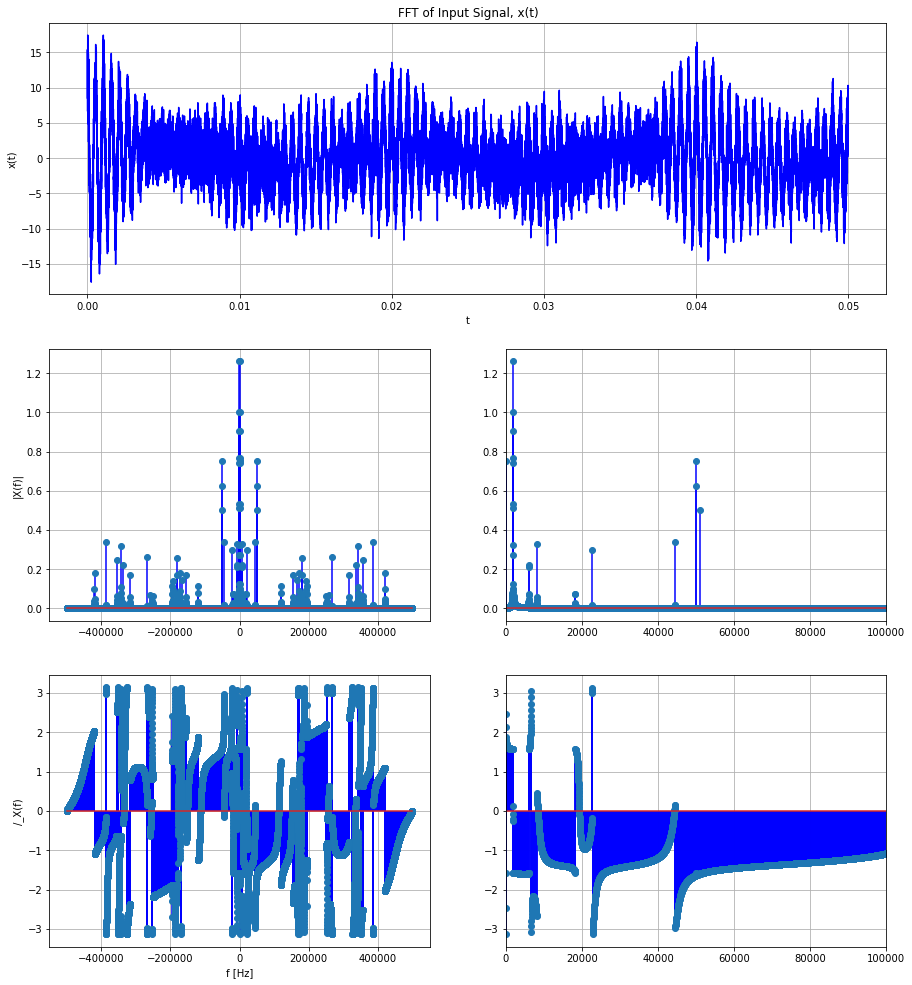
\includegraphics[width=\linewidth]{NISFFT.png}
  \caption{Noisy Input Signal + FFT}
  \label{fig: NISFFT}
\end{figure}
\begin{figure}[h!]
  \centering
  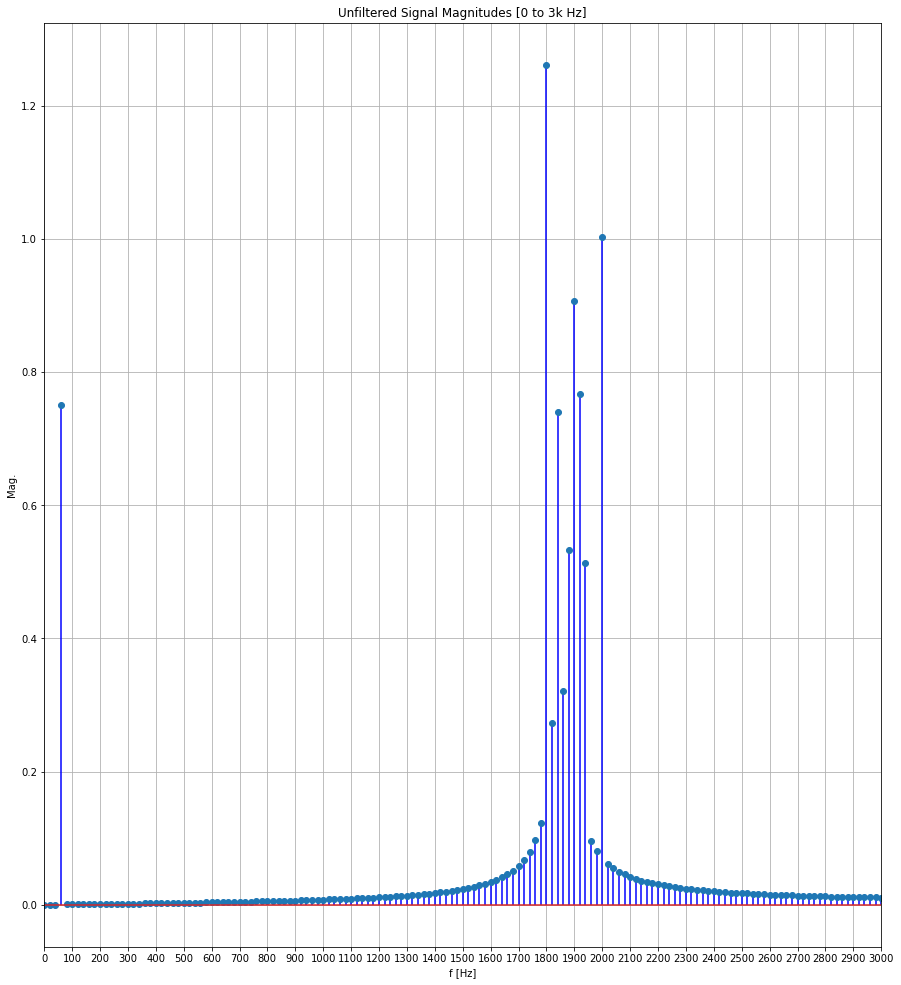
\includegraphics[width=\linewidth]{UISM.png}
  \caption{Noisy Input Signal Magnitudes (Reduced Freq. Range)}
  \label{fig: UISM}
\end{figure}
\begin{figure}[h!]
  \centering
  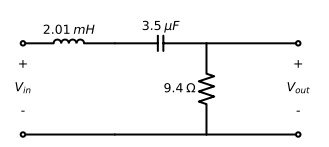
\includegraphics[scale=1]{Filter.png}
  \caption{Filter Design}
  \label{fig: Filter}
\end{figure}
\begin{figure}[h!]
  \centering
  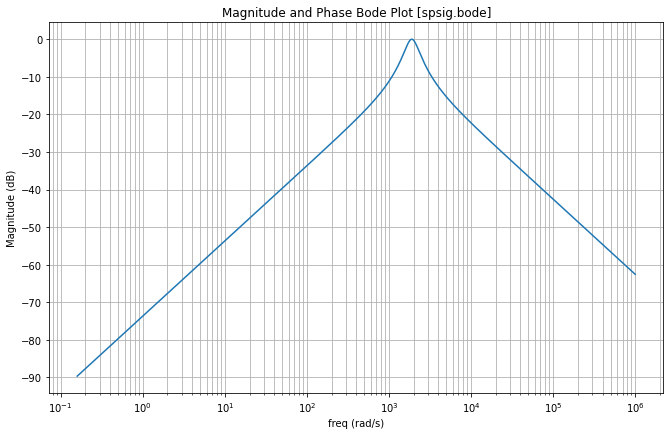
\includegraphics[width=\linewidth]{FRFB.png}
  \caption{Filter Full Range Magnitude Bode Plot}
  \label{fig: FRFB}
\end{figure}
\begin{figure}[h!]
  \centering
  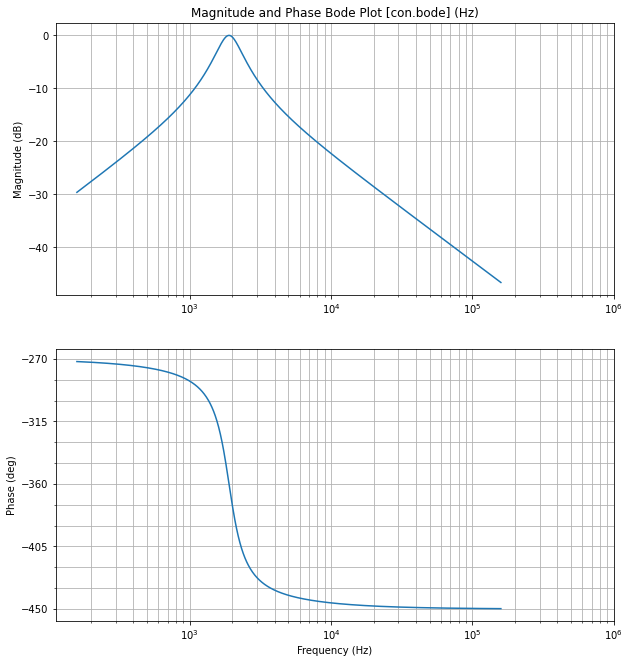
\includegraphics[width=\linewidth]{MPFB.png}
  \caption{Filter Partial Range Magnitude + Phase Bode Plot}
  \label{fig: MPFB}
\end{figure}
\begin{figure}[h!]
  \centering
  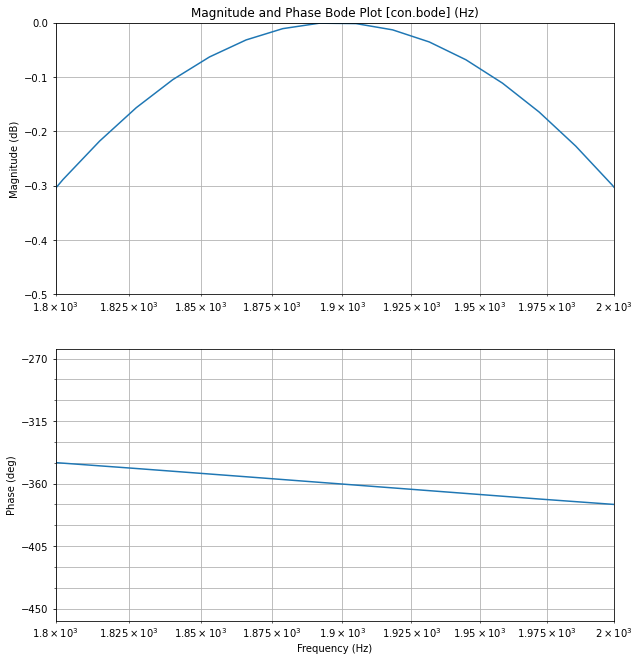
\includegraphics[width=\linewidth]{IRFB.png}
  \caption{Filter Input Range Magnitude + Phase Bode Plot}
  \label{fig: IRFB}
\end{figure}
\begin{figure}[h!]
  \centering
  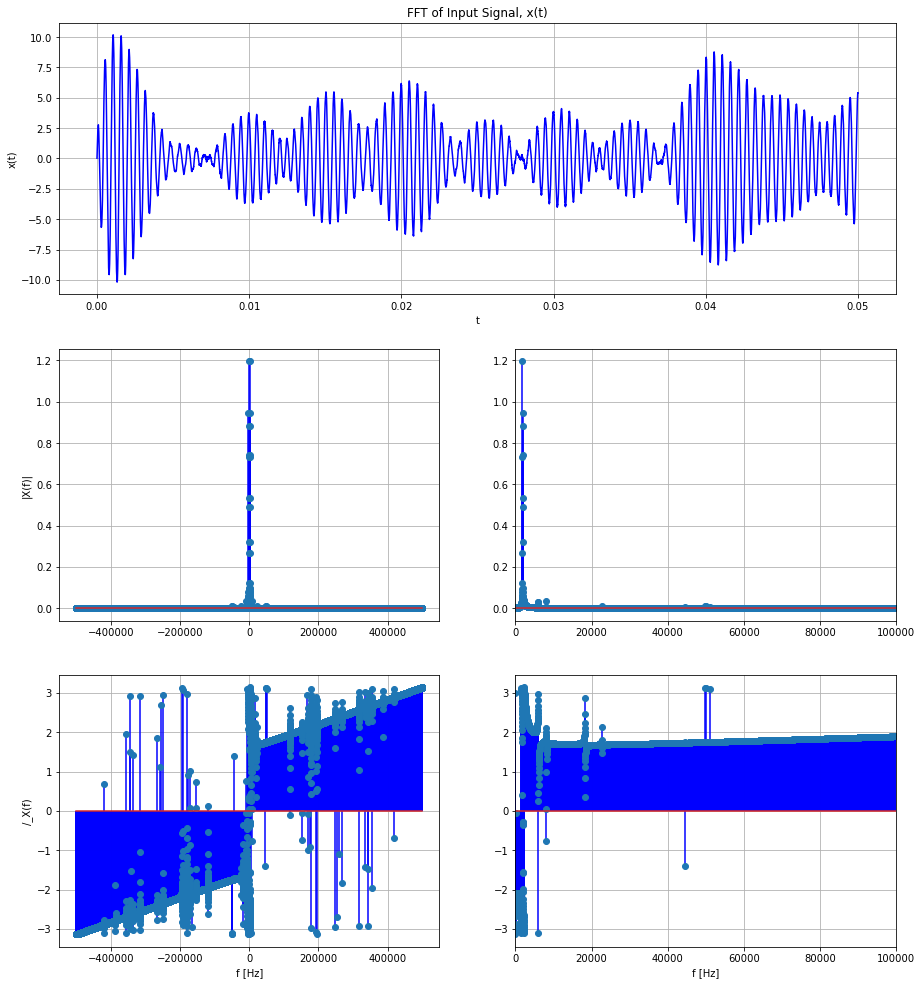
\includegraphics[width=\linewidth]{FISFFT.png}
  \caption{Filtered Input Signal + FFT}
  \label{fig: FISFFT}
\end{figure}
\begin{figure}[h!]
  \centering
  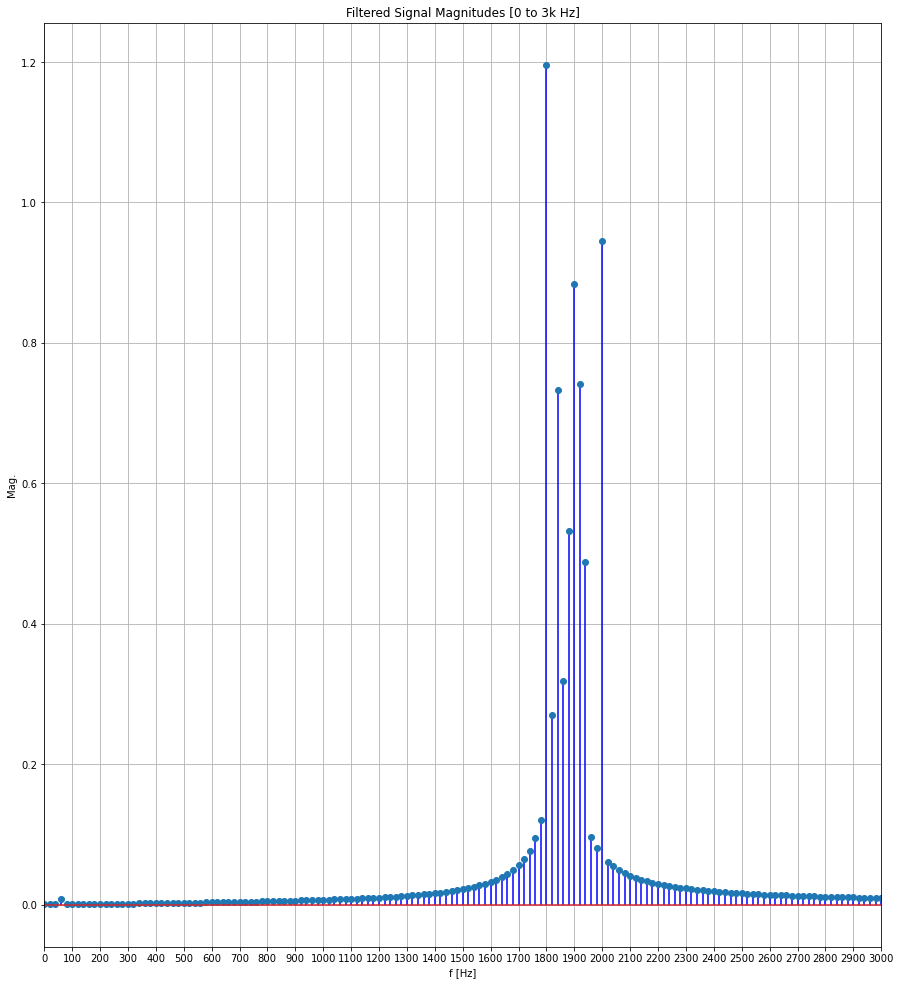
\includegraphics[width=\linewidth]{FISM.png}
  \caption{Filtered Input Signal Magnitudes (Reduced Freq. Range)}
  \label{fig: FISM}
\end{figure}

\section{Error Analysis}\label{section: ErAn}
No sources of error were seen throughout this lab.

\section{Questions}\label{section: Questions}
\begin{enumerate}
  \item Earlier this semester, you were asked what you personally wanted to get out of taking this
  course. Do you feel like that personal goal was met? Why or why not?
  \begin{itemize}
    \item I feel strongly that the personal goal I set at the beginning of this semester was met. I have built my skills in using Python
    to perform post-processing on signals and general mathematics, etc. I have used Python as an aid to verify results of homework questions 
    throughout this course which has been very useful and I think it shows how my goal has been accomplished. 
  \end{itemize}
\end{enumerate}
\section{Conclusion}
In conclusion, I feel this lab was very successful. I feel this lab was a great conglomeration of many concepts
taught throughout the course and it was fun to solve a problem on my own with little hand holding from the lab handout.
All in all, I am very satisfied with what this lab has taught me and feel it was an excellent use of time.
\newpage
\thispagestyle{customblank}
\section{Attachments}\label{section: Attachments}
\centering\begin{enumerate}
  \item Filter design scratch-work
\end{enumerate}
\vspace*{\fill}

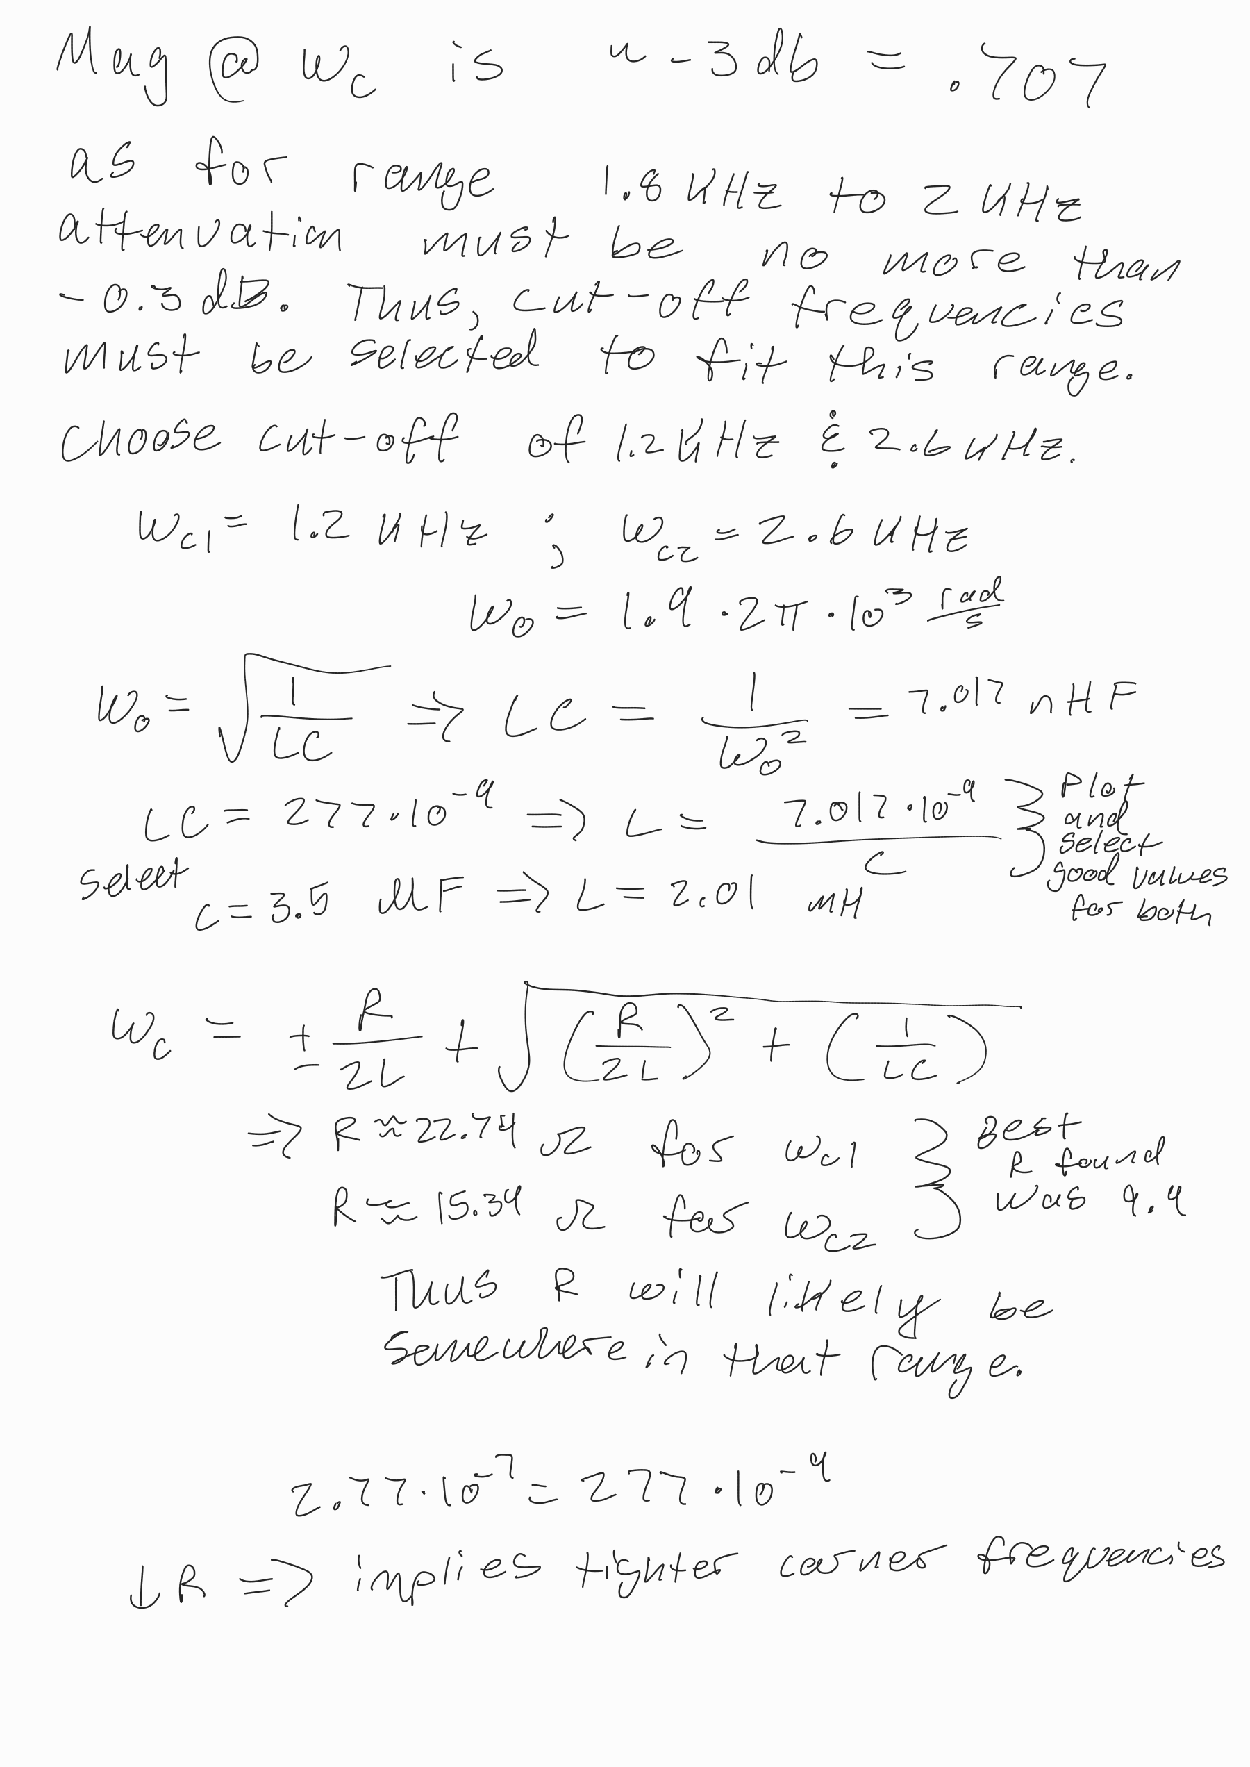
\includepdf[pages=1, offset=1in -1in]{./attachments/lab12.pdf}
% \includepdf[pages=3, offset=1in -1in]{./attachments/lab5.pdf}

% \begin{thebibliography}{111} 
% \thispagestyle{customplain}

% \end{thebibliography}
\end{document}
%This template was created by Roza Aceska.